\documentclass[12pt,a4paper,openany,smallheadings,headinclude,headsepline,final]{scrreprt}
\usepackage[utf8]{inputenc}
\usepackage[english]{babel}
\usepackage[pdftex]{graphicx}
\usepackage{makeidx}
\usepackage[T1]{fontenc}
\usepackage{tabularx}
\usepackage{float}
\usepackage{caption}
\usepackage{listings}
\usepackage{fancyhdr}
\usepackage{color}
\usepackage[bookmarks,colorlinks=true]{hyperref}

\begin{document}
\pagestyle{headings}

\definecolor{dkgreen}{rgb}{0,0.6,0}
\definecolor{gray}{rgb}{0.5,0.5,0.5}
\definecolor{mauve}{rgb}{0.58,0,0.82}
\lstset{ 
basicstyle=\footnotesize\ttfamily,
keywordstyle=\color{blue},
commentstyle=\color{dkgreen},
stringstyle=\color{mauve},
}
\parindent 0cm
\parskip 0.2cm

%\title{ZPUino User Manual}
%\author{Alvaro Lopes}
%\maketitle
\begin{titlepage}
\begin{center}
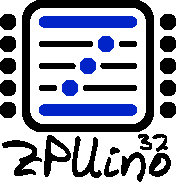
\includegraphics[width=10cm]{zpuino32.pdf}
\vskip 2cm plus 1cm
\huge{\bfseries{ZPUino User Manual}}
\vskip 1cm plus 1cm
\large{\bfseries{Version 1.0.1}}
\end{center}

\end{titlepage}

\tableofcontents
\clearpage

\chapter{Release Notes}

\section{Version 1.0.1}

This release is a minor release, with a few optimization features.

\subsection*{Changes to the HDL Core}
\begin{itemize}
\item The multiplier and shifter are now merged together.
\item Added a new ZPU (optional) instruction, FMUL16, opcode (01h), which performs a fixed-point 16:16 multiplication
\item Multiplier is now signed instead of unsigned
\item SPI controller is now able to do 16, 24 and 32-bit transfers
\item UART now has a bit depicting if all transmission has ended. Needed to fix a bug when your sketch changed baudrate and it was still transmitting.
\end{itemize}

\subsection*{IDE/Code}
\begin{itemize}
\item Updated UARTSTATUS register index
\item IDE now reports a better size for sketches, including program and code size.
\item Removed misinclusion of <new> in some headers
\item IDE can now build and include asssembly (.S) files in the sketch folder
\end{itemize}

\subsection*{Boards}
\begin{itemize}
\item SPI interface is now directly connected on most boards, so to speed up sampling.
\item Add new board (Papilio One 250 with extra 2Kb RAM). All P1 250 are compatible.
\end{itemize}

\subsection*{Libraries}
\begin{itemize}
\item SmallFS was updated to use the new SPI multibyte transfer sizes.
\end{itemize}

\section{Version 1.0.0}

This release is a major release!. Many many changes were done to all components, and not all of them are
depicted here. Please refer to git changelogs for more detail.

\subsection*{Changes to the HDL Core}

\begin{itemize}
\item New ZPU core - ZPU Extreme!
\item Most cores are now Wishbone compatible.
\item New timer implementation 
\item All IO devices were pushed to the top level module, to ease customization 
\end{itemize}

\subsection*{IDE/Code}

\begin{itemize}
 \item New IDE based on Arduino 1.0
 \item Upload-to-RAM feature (control-click on Upload button!!!)
 \item Code is now smaller due to new toolchain features
 \item Some common functions are now exported by the bootloader, to reduce code size.
 \item Some functions have now assembly implementations for speed.
\end{itemize}

\subsection*{Boards}
\begin{itemize}
 \item New board: Papilio Plus S6LX4
 \item New board: Papilio Plus S6LX9
 \item New board: Nexys2 S3E1200 (thanks to Paul Urbanus)
 \item New board variants!
\end{itemize}

\subsection*{Libraries}
\begin{itemize}
 \item Small fixes here and then.
\end{itemize}

\subsection*{Other/Contributed}
\begin{itemize}
\item SID HDL implementation
\item Pokey HDL implementation
\item YM2149 HDL implementation
\item Audiomixer and simple sigmadelta
\item OpenCores I2C
\end{itemize}



\chapter{ZPUino}
ZPUino is a SoC (System-on-a-Chip) based on Zylin's ZPU 32-bit processor core.

\subsection{What is inside ZPUino}

Hardware-wise, ZPUino currently integrates the following devices:

\begin{itemize}
\item ZPU Extreme Core, a modified ZPU core
\item One or two UART
\item Two SPI interfaces
\item A 16-bit and a 24-bit timer.
\item One TSC (Time Stamp Counter)
\item 128-bit GPIO interface
\item Interrupt Controller
\item Two SigmaDelta outputs
\item Peripheral Pin Select
\item VGA (optional)
\end{itemize}

Software-wise, it supports the following features:

\begin{itemize}
\item 4Kb Bootloader, which includes required emulation code for ZPU.
\item Bootstraps code from program flash (shadows into FPGA blockram)
\item Serial programming of program flash.
\end{itemize}

\subsection{Where does it run}
First implementation was done on Spartan3E 500 (-4), on a S3E Starter Kit, with a M25P16 SPI flash ROM and 32Kbytes RAM.\\
Right now it runs on other many boards, see chapter \ref{boards} for more information. \\
unning speed: up to 100MHz, 96MHz recommended.

\subsection{IO Device features}

UART features:
\begin{itemize}
\item 16-bit prescaler
\item 2048-byte deep receive FIFO. (16 byte in reduced implementations)
\end{itemize}

SPI features:
\begin{itemize}
\item Two independent SPI master controllers
\item Programmable prescaler
\item Configurable CPOL
\item Configurable SRE (Sample on Rising Edge)
\item 8, 16, 24 and 32-bit transmission modes, 4 byte (32 bit) receive register.
\item Configurable blocking operation
\end{itemize}

Timer features:
\begin{itemize}
\item Two independent timers
\item 10-bit prescaler
\item 16-bit and 24-bit counter
\item Count-up and Count-down mode
\item 16-bit Compare register
\item Clear on Compare match support
\item Interrupt support on Compare Match
\item Output compare Registers to GPIO pin (allows PWM)
\end{itemize}

GPIO features:
\begin{itemize}
\item Up to 128 GPIO entries
\item Bi-directional (tristate) configuration
\end{itemize}

SigmaDelta features:
\begin{itemize}
\item Two 16-bit channel
\item Runs at system clock speed
\item Configurable endianness
\end{itemize}

PPS (Peripheral pin select) features:
\begin{itemize}
\item Map every device pin to any GPIO pin
\item Fully configurable in run-time
\end{itemize}

VGA features:
\begin{itemize}
\item HQVGA (160x120), using 800x600@75Hz output.
\item 8-bit color (3 bits red, 3 bits green, 2 bits blue).
\item Integrated programable character ram (8x8)
\end{itemize}

ZPUino programmer:
\begin{itemize}
\item 1Mbps programming speed
\item Supports programming both sketches and FPGA bitfile [if ZPUino bootloader already loaded]
\item Support for upload-to-ram
\end{itemize}

\subsection{Hardware support}

Currently ZPUino should run on any Spartan3E FPGA (from 250 and beyond), and Spartan6 FPGA (LX4 and beyond). \\
List of flash devices currently supported by programmer:
\begin{itemize}
\item ST M25P16
\item SST SST25VF040B
\item ATMEL AT45DB081D
\end{itemize}
Other flash might be supported. Specifically flash from same series, but with different capacities, can be easily added to programmer.
For other flash vendors or models contact us by e-mail.


%\chapter{Acknowledgments}

A few credits and acknowledgments are due for all ZPUino development. I surely hope
all those who somehow contributed to ZPUino with ideas, code, boards and criticism
are depicted here. If you believe you did contribute, and you are not listed, please
drop me a note, and I'll update the document.

\begin{description}
\item{\O yvind Harboe and Zylin} \hfill \\
A huge thanks to Zylin and \O yvind, for their ZPU processor. This would not exist unless for their
work. Always supportive from the beginning. 

\item{The ZPU guys} \hfill \\
A special thanks to all ZPU guys. I'll try to enumerate all of them, but some might be missing:
\begin{description}
\item{Bert Lange} \hfill \\ Maintainer (with me) of ZPU official repository. Fantastic work.
\item{Martin Strubel} \hfill \\ The debugging guy, with lots of ideas.
\item{Rick Collins} \hfill \\ The HDL/Hardware man. 
\item{Carl Hacken\"as} \hfill \\ The compiler man. 
\end{description}

\item{The afficcionados}
\item{The supporters}


\end{description}


\section{Overview}
\includegraphics[width=16cm]{zpuino-overview2.pdf}


\chapter{Peripheral Pin Select}
This information relates to ZPUino 1.0 release. Other releases might have different specs. \\


ZPUino includes a feature which is called Peripheral Pin Select (in short, PPS). 
PPS allows you to map every device input or output pin (such as SPI clock and SPI data lines) to 
each individual pin (GPIO), thus not requiring you to perform synthesis and P\&R each time you want to use
a device on a different IO pin. \\
To simplify things, three methods are supplied to manipulate PPS:

\begin{lstlisting}[language=C++]
void pinModePPS(int pin, int value);
void outputPinForFunction(unsigned int pin,unsigned int function);
void inputPinForFunction(unsigned int pin,unsigned int function);
\end{lstlisting}

Three register blocks exist to configure how pin selection is done. These are called $GPIOPPSIN$,
$GPIOPPSOUT$ and $GPIOPPSMAP$. The above functions manipulate these registers.


\section{Redirecting output}
In order to direct any peripheral output to a GPIO pin, you have to:

\begin{itemize}
\item Configure the GPIO pin as output;
\item Enable PPS on selected GPIO pin;
\item Configure $GPIOPPSOUT$ (outputPinForFunction) to the peripheral signal
\end{itemize}

\subsection{Examples}
The following example maps Sigma Delta 1st channel into GPIO pin number 30:

\begin{lstlisting}[language=C++]
void setup(void)
{
  // Configure pin as output
  pinMode(30,OUTPUT); 
  // enable PPS on this pin
  pinModePPS(30,HIGH); 
  // Map SigmaDelta channel 1 to pin 30
  outputPinForFunction(30, IOPIN_SIGMADELTA1); 
}
\end{lstlisting}
Note that you can use GPIO aliases for your board instead of GPIO number. See your board specific documentation.

\section{Redirecting input}
In order to direct GPIO input into any peripheral, you have to:
\begin{itemize}
\item Configure the GPIO pin as input;
\item Configure $GPIOPPSIN$ (inputPinForFunction) to the peripheral signal;
\end{itemize}

Note that for input you don't need to enable PPS on the pin using $pinModePPS$.\\

\subsection{Examples}
The following example maps USPI MISO signal (Master-In Slave-out) to GPIO pin number 10:
\begin{lstlisting}[language=C++]
void setup(void)
{
  // Configure pin as input
  pinMode(10,INPUT); 
  // Map pin 30 to USPI MISO
  inputPinForFunction(10, IOPIN_USPI_MISO); 
}
\end{lstlisting}


\chapter{IO Modules}
ZPUino comes with a few IO modules you can use. You can also add other modules, since ZPUino is Wishbone compliant.\\
IO accesses in ZPUino are done using MMIO (Memory Mapped IO).\\
In ZPUino IO devices are connected to the IO module in slots, and can be accessed using the "C" macro $IO\_SLOT(x)$, where $x$
depicts the slot ID for the module.\\


Registers in each IO slot can be accessed using the "C" $REGISTER(base,x)$ macro, 
where $base$ depicts the MMIO address, and $x$ depicts the register index.\\

For example, to write to the 3rd register of IO slot 9, you can do it the following way:
\begin{lstlisting}[language=C++]
void writetodevice(unsigned int value) {
  // Write to 3rd register on IO slot 9 
  REGISTER(IO_SLOT(9),3) = value;
}
\end{lstlisting}

See the board specific documentation for current allocation of IO modules.

\section{GPIO}
\subsection{HDL sources and modules}

\subsubsection{HDL instantiation template}
\begin{lstlisting}[language=VHDL]
component zpuino_gpio is
  generic (
    gpio_count: integer := 32
  );
  port (
    wb_clk_i: in std_logic;
    wb_rst_i: in std_logic;
    wb_dat_o: out std_logic_vector(wordSize-1 downto 0);
    wb_dat_i: in std_logic_vector(wordSize-1 downto 0);
    wb_adr_i: in std_logic_vector(maxIObit downto minIObit);
    wb_we_i:  in std_logic;
    wb_cyc_i: in std_logic;
    wb_stb_i: in std_logic;
    wb_ack_o: out std_logic;
    wb_inta_o:out std_logic;

    spp_data: in std_logic_vector(gpio_count-1 downto 0);
    spp_read: out std_logic_vector(gpio_count-1 downto 0);

    gpio_o:   out std_logic_vector(gpio_count-1 downto 0);
    gpio_t:   out std_logic_vector(gpio_count-1 downto 0);
    gpio_i:   in std_logic_vector(gpio_count-1 downto 0);

    spp_cap_in:  in std_logic_vector(gpio_count-1 downto 0);
    spp_cap_out:  in std_logic_vector(gpio_count-1 downto 0)
  );
end component;
\end{lstlisting}
\subsubsection{Compliance}
The GPIO module is wishbone compatible, in non-pipelined mode.
\subsubsection{Generics}

\begin{description}
\item{gpio\_count} \hfill \\ 
Number of GPIO (1 to 128)
\end{description}

\subsubsection{Source files}

All GPIO system is implemented in \emph{zpuino\_gpio.vhd}.

\subsubsection{PPS capability}

Some pins can have their PPS capability disabled in order to reduce complexity in some designs. The two inputs $spp\_cap\_in$ and
$spp\_cap\_out$ can be manipulated so that some pins have or not in/out PPS capabilities.

\subsection{Location}
GPIO are located in IOSLOT 2.

\subsection{Registers}

Two bits can be manipulated for each GPIO pin, a tristate bit and an output bit. GPIO uses up to 4 32-bit individual
registers in order to map all 128-bits. Note that the actual number of GPIO available is board dependant.

\subsubsection{GPIODATA register}
GPIODATA is actually a 4-word register. Each bit maps a single GPIO input/output. If the GPIO is configured as an output (see 
$GPIOTRIS$ register for input/output selection) writing a 0 or 1 to a specific bit will cause the underlying pin to become 0 or 1 
(except if pin is currently mapped to a peripheral - see PPS for more details). When read it will depict the values at an input (if
the pin is configured as an input) or the current output value if it's configured as an output.
\begin{table}[H]
\begin{center}
\begin{tabularx}{14cm}{X}
31 \hfill 0 \\
\hline
\multicolumn{1}{|c|}{\tiny GPIODATA [31:0]} \\
\hline
63 \hfill 32 \\
\hline
\multicolumn{1}{|c|}{\tiny GPIODATA [63:32]} \\
\hline
95 \hfill 64 \\
\hline
\multicolumn{1}{|c|}{\tiny GPIODATA [95:64]} \\
\hline
127 \hfill 96 \\
\hline
\multicolumn{1}{|c|}{\tiny GPIODATA [127:96]} \\
\hline
\end{tabularx}
\caption{GPIODATA register}
\end{center}
\end{table}

\subsubsection{GPIOTRIS register}
$GPIOTRIS$ is actually a 4-word register. When a bit is set to one, the GPIO becomes an input (it will be tristated).

\begin{table}[H]
\begin{center}
\begin{tabularx}{14cm}{X}
31 \hfill 0 \\
\hline
\multicolumn{1}{|c|}{\tiny GPIOTRIS [31:0]} \\
\hline
63 \hfill 32 \\
\hline
\multicolumn{1}{|c|}{\tiny GPIOTRIS [63:32]} \\
\hline
95 \hfill 64 \\
\hline
\multicolumn{1}{|c|}{\tiny GPIOTRIS [95:64]} \\
\hline
127 \hfill 96 \\
\hline
\multicolumn{1}{|c|}{\tiny GPIOTRIS [127:96]} \\
\hline
\end{tabularx}
\caption{GPIOTRIS register}
\end{center}
\end{table}



\subsection{Software}

GPIO pins should be manipulated using the Arduino-like functions $digitalWrite()$, $digitalRead()$ and $pinMode()$.
Additionaly GPIO can be bound to devices using PPS (Peripheral Pin Select).
                                   
You can also use the following "C" macros if needed. Each pin block is 32-bit wide:

\begin{description}
\item{GPIODATA(x)} \hfill \\ GPIODATA for pin block x
\item{GPIOTRIS(x)} \hfill \\ GPIOTRIS for pin block x
\end{description}

\section{Timers}
ZPUino includes two generic timers, which are able to generate PWM signals. 
The default implementation includes a 16-bit timer with prescaler and TSC, and a second 24-bit timer with no prescaler nor TSC.
The PWM controls of the 2nd timer are double buffered.

\subsection{HDL sources and modules}

\subsubsection{HDL instantiation template}
\begin{lstlisting}[language=VHDL]
component zpuino_timers is
  generic (
    A_TSCENABLED: boolean := false;
    A_PWMCOUNT: integer range 1 to 8 := 2;
    A_WIDTH: integer range 1 to 32 := 16;
    A_PRESCALER_ENABLED: boolean := true;
    A_BUFFERS: boolean :=true;
    B_TSCENABLED: boolean := false;
    B_PWMCOUNT: integer range 1 to 8 := 2;
    B_WIDTH: integer range 1 to 32 := 16;
    B_PRESCALER_ENABLED: boolean := false;
    B_BUFFERS: boolean := false
  );

  port (
    wb_clk_i: in std_logic;
    wb_rst_i: in std_logic;
    wb_dat_o: out std_logic_vector(wordSize-1 downto 0);
    wb_dat_i: in std_logic_vector(wordSize-1 downto 0);
    wb_adr_i: in std_logic_vector(maxIObit downto minIObit);
    wb_we_i:  in std_logic;
    wb_cyc_i: in std_logic;
    wb_stb_i: in std_logic;
    wb_ack_o: out std_logic;
    wb_inta_o:out std_logic;
    wb_intb_o:out std_logic;
    
    pwm_A_out: out std_logic_vector(A_PWMCOUNT-1 downto 0);
    pwm_B_out: out std_logic_vector(B_PWMCOUNT-1 downto 0)
  );
end component;
\end{lstlisting}

\subsubsection{Compliance}
The Timer module is wishbone compatible, in non-pipelined mode.

\subsubsection{Generics}

There are two sets of generics, one for each timer (timer A and B)

\begin{description}
\item{TSCENABLED} \hfill \\ Set if TSC (TimeStamp Counter) is enabled on timer A/B(default: false)
\item{PWMCOUNT} \hfill \\ Number of PWM outputs for timer A/B (default: 2)
\item{WIDTH} \hfill \\ Timer A/B width, in bits (default: 16)
\item{PRESCALER\_ENABLED} \hfill \\ Set if prescaler is enabled for timer A/B (default: true for timer A, false for timer B)
\item{BUFFERS} \hfill \\ Set if double-buffering of PWM registers is enabled on this timer (default: false for timer A, true for timer B)
\end{description}


\subsubsection{Source files}

ZPUino Timers are composed of the following source modules:

\begin{table}[h!]
\begin{center}
\begin{tabularx}{10cm}{ll}

zpuino\_timers.vhd & Top level Timers module \\
timer.vhd & Timer module \\
prescaler.vhd & Prescaler module
\end{tabularx}
\end{center}
\caption{Timer source files}
\end{table}

\subsection{Location}

Timer registers are usualy located in IOSLOT 3.

\subsection{Registers}

\subsubsection{TMRxCTL register}

TMRxCTL is located at offset $0$ for the first timer, and offset $64$ for the second timer.

\begin{table}[H]
\begin{center}
\begin{tabularx}{14cm}{Xcccccccc}
31 \hfill 11 & 10 \hfill 9 & 8 & 7 & 6  \hfill 4 & 3 & 2 & 1 & 0  \\
\hline
\multicolumn{1}{|c|}{\tiny rsvd} & 
\multicolumn{1}{|c|}{\tiny TMRUPDP} &
\multicolumn{1}{|c|}{\tiny rsvd\footnote{On pre-1.0 release, this used to be a OCREN register, but it's no longer used}} &
\multicolumn{1}{|c|}{\tiny TMRINTR} &
\multicolumn{1}{|c|}{\tiny TMRPRES} &
\multicolumn{1}{|c|}{\tiny TMRIEN} &
\multicolumn{1}{|c|}{\tiny TMRDIR} &
\multicolumn{1}{|c|}{\tiny TMRCCM} &
\multicolumn{1}{|c|}{\tiny TMREN}  \\
\hline
\end{tabularx}
\caption{TMRxCTL register}
\end{center}
\end{table}


\begin{description}

\item{0 - TMREN [RW]} \hfill \\
Timer Enable. When set to '1', timer will count either up or down, depending on $TMRDIR$ value.

\item{1 - TMRCCM [RW]} \hfill \\
Timer Clear on Compare Match. If this bit is set, whenever $TMRCNT$ matches $TMRCMP$ the current
value of $TMRCNT$ will be set to zero.

\item{2 - TMRDIR [RW]}\hfill \\
Timer count direction. If this bit is set, then at every timer tick the value of $TMRCNT$ will be incremented. If this
bit is not set, then $TMRCNT$ value will be decremented instead.

\item{3 - TMRIEN [RW]} \hfill \\
Timer Interrupt Enable. When this bit is set and $TMRINTR$ is not set, an interrupt is generated whenever 
$TMRCNT$ matches $TMRCMP$.
To rearm interrupt $TMRINTR$ must be cleared before exiting the ISR routine.

\item{[6-4] TMRPRES [RW]} \hfill \\
Timer prescaler. The timer prescale has 3 bits. See table \ref{timerprescaler} for more details on the prescaler value.
                 
\item{7 - TMRINTR [RW]} \hfill \\
Timer Interrupt. This bit is set whenever an interrupt occurs. It needs to be cleared in software to re-enable this interrupt
source.

\item{8 - Reserved} \hfill \\
Reserved.

\item{[10:9] - TMRUPDP [RW]} \hfill \\
Timer PWM update policy. See table \ref{updatepolicy} for details.

\end{description}


\subsubsection{TMRxCNT}
TMRxCNT is located at offset $1$ for the first timer, and offset $65$ for the second timer. \\
Current timer counter value. This is a read/write register.

\subsubsection{TMRxCMP}

TMRxCMP is located at offset $2$ for the first timer, and offset $66$ for the second timer. \\
Current timer compare value. This is a read-write register.

\subsubsection{TMRxTSC}

TMRxCMP is located at offset $3$ for the first timer, and offset $67$ for the second timer. \\
Timestamp Counter. This register is only available in the first timer (by omission). It's also known as $TIMERTSC$.
This register is incremented at each clock cycle, and is 32-bit wide. It's a read-only register.

\subsection{PWM registers}

The PWM output, is, unlike common PWM implementations, controlled by a LOW and a HIGH register. This allows for 
more precise operation. \\
The exact location of PWM registers are a bit complex, since each timer might have zero or more PWM outputs.
The address for PWM output $Y$ of timer $X$ can be computed by the following equation:

\begin{displaymath}
TMRxPWMBASE = ( 64 \times X) + 32 + ( 4 \times Y )
\end{displaymath}

Use the provided "C" macros whenever possible. See section \ref{timersoftware} for more details.

\subsubsection{TMRxPWMLOW}
TMPxPWMLOW is located at offset $0$ from TMRxPWMBASE.\\
Low PWM compare value. If $TMRxCNT$ is higher or equal this value, the PWM will output 0. It's a write-only register.
\subsubsection{TMRxPWMHIGH}
TMPxPWMLOW is located at offset $1$ from TMRxPWMBASE.\\
High PWM compare value. If $TMRxCNT$ is lower than this value, the PWM will output 1. It's a write-only register.
\subsubsection{TMRxPWMCTL}
TMPxPWMLOW is located at offset $2$ from TMRxPWMBASE.\\
PWM control bits. It's a write-only register.

\begin{table}[H]
\begin{center}
\begin{tabularx}{14cm}{Xc}
31 \hfill 1 & 0  \\
\hline
\multicolumn{1}{|c|}{Reserved} & 
\multicolumn{1}{|c|}{PWMxEN}  \\
\hline
\end{tabularx}
\caption{TMRxPWMCTL register}
\end{center}
\end{table}

\begin{description}

\item{0 - PWMxEN} \hfill \\
PWM enable
\end{description}





\subsection{Timer prescaler}
When enabled, the timer prescaler divides the main clock according to table \ref{timerprescaler}.

\begin{table}[H]
\begin{center}
\begin{tabularx}{6cm}{|c|c|}
\hline
Prescaler value & Clock divider \\
\hline
000 & 1 \\
\hline
001 & 2 \\
\hline
010 & 4 \\
\hline
011 & 8 \\
\hline  
100 & 16  \\
\hline
101 & 64  \\
\hline
110 & 256 \\
\hline
111 & 1024 \\
\hline
\end{tabularx}
\caption{Timer prescaler values}\label{timerprescaler}
\end{center}
\end{table}

\subsection{Timer PWM update policy}
Sometimes is desirable to use a double-buffering technique when manipulating PWM parameters, to avoid 
them changing at unwanted time.

\begin{table}[H]
\begin{center}    
\begin{tabular}{|c|c|}
\hline
UPDP value & Update Policy \\
\hline
00 & UPDATE NOW \\
\hline
01 & UPDATE ON ZERO SYNC \\
\hline
10 & UPDATE LATER \\
\hline
11 & Reserved \\
\hline
\end{tabular}
\caption{PWM update policy}\label{updatepolicy}
\end{center}
\end{table}

\begin{description}
\item{UPDATE NOW} \hfill \\
Update PWM values as you write them.
\item{UPDATE ON ZERO SYNC} \hfill \\
Update PWM values when the timer counter reaches 0. Until then the new PWM values will stay on the double buffer.
\item{UPDATE LATER} \hfill \\
Don't update PWM values, just update the double buffer.
\end{description}

For precise PWM synchronization, do:
\begin{itemize}
\item Set update policy to UPDATE LATER. 
\item Change the PWM parameters at will.
\item Set update policy to UPDATE ON ZERO SYNC. When timer counter reaches 0 (or overflows), all PWM will be set synchronously.
\end{itemize}

\subsection{Software}\label{timersoftware}
As of ZPUino 1.0, no software classes are implemented to manipulate the timer, meaning you have to write directly to its registers. \\
\subsubsection{Setting up a timer interrupt}

The following example shows how to use interrupts with Timer 0. 
Timer is set up for a 100KHz operation with interrupts enabled.
\begin{lstlisting}[language=C++]
void _zpu_interrupt()
{
  if (TMR0CRL & _BV(TCTLIF)) { /* Interrupt comes from timer 0 */
                
    /* do something here... */
                
    /* Clear the interrupt flag on timer register */
    TMR0CTL &= ~_BV(TCTLIF);
  }
}

void setup()
{
  unsigned frequency = 100000;
        
  TMR0CNT = 0;  /* Clear timer counter */
  TMR0CMP = (CLK_FREQ / frequency) - 1; /* Set up timer, no prescaler */
  TMR0CTL = _BV(TCTLENA)|_BV(TCTLCCM)|_BV(TCTLDIR)|_BV(TCTLIEN);

  INTRMASK = _BV(INTRLINE_TIMER0); /* Enable timer 0 interrupt on mask */
  INTRCTL = _BV(INTREN); /* Globally enable interrupts */
}
\end{lstlisting}




\subsubsection{PWM}
A few macros are provided to ease PWM register access: \\

\begin{description}
\item{TMR0PWMLOW(x)} \hfill \\ PWMLOW register on timer 0, for PWM output x
\item{TMR0PWMHIGH(x)}\hfill \\ PWMHIGH register on timer 0, for PWM output x
\item{TMR0PWMCTL(x)} \hfill \\ PWMCTL register on timer 0, for PWM output x

\item{TMR1PWMLOW(x)} \hfill \\ PWMLOW register on timer 1, for PWM output x
\item{TMR1PWMHIGH(x)}\hfill \\ PWMHIGH register on timer 1, for PWM output x
\item{TMR1PWMCTL(x)} \hfill \\ PWMCTL register on timer 1, for PWM output x

\end{description}

\section{UART}

ZPUino UART is a generic UART implementation, with a 16x oversampling filter. Only $8n1$ 
data format is supported (1 start bit, 8 data bits, 1 stop bit, no
parity). With a $96Mhz$ clock, baud rates up to $3Mbit$ can be used with perfect timing alignment.
\subsection{HDL sources and modules}

\subsubsection{HDL instantiation template}

\begin{lstlisting}[language=VHDL]
component zpuino_uart is
  generic (
    bits: integer := 11
  );
  port (
    wb_clk_i: in std_logic;
    wb_rst_i: in std_logic;
    wb_dat_o: out std_logic_vector(wordSize-1 downto 0);
    wb_dat_i: in std_logic_vector(wordSize-1 downto 0);
    wb_adr_i: in std_logic_vector(maxIObit downto minIObit);
    wb_we_i:  in std_logic;
    wb_cyc_i: in std_logic;
    wb_stb_i: in std_logic;
    wb_ack_o: out std_logic;
    wb_inta_o:out std_logic;

    enabled:  out std_logic;
    tx:       out std_logic;
    rx:       in std_logic
  );
end component;
\end{lstlisting}



\subsubsection{Compliance}
The UART module is wishbone compatible, in non-pipelined mode.





\subsubsection{Generics}

\begin{description}
\item{bits} \hfill \\ Number of RX FIFO address bits
\end{description}
UART FIFO size will be $2^{bits}$ bytes wide. Default FIFO address size is 11 bits ($2^{11}=2048$ bytes)

\subsubsection{Source files}

ZPUino UART is composed of the following source modules:

\begin{table}[h!]
\begin{center}
\begin{tabularx}{10cm}{ll}

zpuino\_uart.vhd & Top level UART module \\
zpuino\_uart\_rx.vhd & UART RX module \\
uart\_brgen.vhd & Baud rate generator \\
zpuino\_uart\_mv\_filter.vhd & RX Majority voting filter \\
tx\_unit.vhd & UART TX module \\
fifo.vhd & UART FIFO module

\end{tabularx}
\end{center}
\caption{UART source files}
\end{table}



\subsection{Location}

UART registers are usualy located in IOSLOT 1.

\subsection{Registers}
UART operation is controlled by three registers, $UARTCTL$, $UARTDATA$ and \\
$UARTSTATUS$.

\subsubsection{UARTCTL register}
The $UARTCTL$ register controls the transmit and receive operation of the UART.

\begin{table}[h!]
\begin{center}
\begin{tabularx}{14cm}{Xcc}
31 \hfill 17 & 16 & 15 \hfill 0  \\
\hline
\multicolumn{1}{|c|}{Reserved} & 
\multicolumn{1}{|c|}{UARTEN} & 
\multicolumn{1}{|c|}{UARTPRES} \\
\hline
\end{tabularx}
\caption{UARTCTL register}\label{UARTCTL}
\end{center}
\end{table}

\begin{description}
\item{16 - UARTEN} \hfill \\
UARTEN bit controls whether UART is enabled or not. When set to 1, UART input
and output will be mapped to appropriate pins. When set to 0 TX and RX will be
disconnected.
\item{[15:0] - UARTPRES} \hfill \\
 UART prescaler (16 bits). See \ref{UART Prescaler} for details.
\end{description}


\subsubsection{UARTDATA register}
The $UARTDATA$ register is used for tranmission and reception of UART data. Reception includes a configurable (synthesis time) FIFO.
Only the lower 8 bits of this register are used.

\begin{table}[H]
\begin{center}
\begin{tabularx}{14cm}{Xc}
31 \hfill 8 & 7 \hfill 0  \\
\hline
\multicolumn{1}{|c|}{Reserved} & 
\multicolumn{1}{|c|}{TXRXD} \\
\hline
\end{tabularx}
\caption{UARTDATA register}
\end{center}
\end{table}

\begin{description}
\item{[7:0] - TXRXD} \hfill \\
 8-bit UART data transmit and receive register.
\end{description}

\subsubsection{UARTSTATUS register}

The $UARTSTATUS$ register contains the current status of UART.


\begin{table}[H]
\begin{center}
\begin{tabularx}{14cm}{Xccc}
31 \hfill 3 & 2 & 1 & 0 \\
\hline
\multicolumn{1}{|c|}{Reserved} &
\multicolumn{1}{|c|}{UARTINTX} &
\multicolumn{1}{|c|}{UARTTXR} &
\multicolumn{1}{|c|}{UARTRXR} \\
\hline
\end{tabularx}
\caption{UARTSTATUS register}
\end{center}
\end{table}

\begin{description}
\item{1 - UARTINTX\footnote{Introduced in 1.0.1 version}} \hfill \\
UART in TX flag. Reads as 1 if the UART is still transmitting any data, 0 otherwise. This bit should be used to wait until
UART has finished transmitting all data, for example when switching the baud rate.
\item{1 - UARTTXR} \hfill \\
UART TX Ready bit. Reads as 1 when there's space in TX FIFO for transmission, 0 otherwise. This bit should be checked before 
attempting transmission over the UART.

\item{0 - UARTRXR} \hfill \\
UART RX Ready bit. Reads as 1 when there's received data in FIFO, 0 otherwise.

\end{description}



\subsection{UART Prescaler}\label{UART Prescaler}
The UART Prescaler divides system clock and provides baud rate generation for RX and TX. 
An additional prescaler of 16 is used by the RX module. Prescaler can be configured by
setting the appropriate bits in the $UARTCTL$ register.

\begin{displaymath}
Prescale = \frac{f_{OSC}}{baudrate \times 16} - 1
\end{displaymath}

\subsection{Software}
Acessing the UART in software can be done using the $HardwareSerial$ class. The default UART module is 
already instantiated as $Serial$.
\subsubsection{Examples}
The following example uses the default $Serial$ object.
\begin{lstlisting}[language=C++]
void setup()
{
    Serial.begin(115200);              /* Set up serial at 115200 baud */
    Serial.println("Hello world!");    /* Write Hello World! to serial */
}
void loop()
{
    if (Serial.available()) {          /* If there is data on the UART... */
        Serial.write( Serial.read() ); /* ... write it back! */
    }
}
\end{lstlisting}

The follwing example uses a custom UART on IOSLOT 9:

\begin{lstlisting}[language=C++]

HardwareSerial mySerial(9); /* New Serial UART on IO SLOT 9 */

void setup()
{
    mySerial.begin(115200);            /* Set up serial at 115200 baud */
    mySerial.println("Hello world!");  /* Write Hello World! to serial */
}
void loop()
{
    if (mySerial.available()) {          /* If there is data on the UART... */
        mySerial.write( Serial.read() ); /* ... write it back! */
    }
}
\end{lstlisting}


\section{CRC16}
The CRC16 module implements a CRC16 engine with configurable polynomial.\\
This module is required. It's used by the bootloader code.
\subsection{HDL sources and modules}
\subsubsection{HDL instantiation template}



\begin{lstlisting}[language=VHDL]
component zpuino_crc16 is
  port (
    wb_clk_i: in std_logic;
    wb_rst_i: in std_logic;
    wb_dat_o: out std_logic_vector(wordSize-1 downto 0);
    wb_dat_i: in std_logic_vector(wordSize-1 downto 0);
    wb_adr_i: in std_logic_vector(maxIOBit downto minIOBit);
    wb_we_i:  in std_logic;
    wb_cyc_i: in std_logic;
    wb_stb_i: in std_logic;
    wb_ack_o: out std_logic;
    wb_inta_o:out std_logic
  );
end component;
\end{lstlisting}



\subsubsection{Compliance}
The CRC16 is wishbone compatible, in non-pipelined mode.


\subsubsection{Source files}
All CRC16 system is implemented in \emph{zpuino\_crc16.vhd}.

\subsection{Location}

\subsection{Registers}

\subsubsection{CRCACC}
The $CRCACC$ register contains the accumulated CRC16 value. It's a read-write register.

\begin{table}[H]
\begin{center}
\begin{tabularx}{14cm}{XX}
31 \hfill 16 & 15 \hfill 0 \\

\hline
\multicolumn{1}{|c|}{Reserved} & 
\multicolumn{1}{|c|}{CRC16ACC}  \\

\hline
\end{tabularx}
\caption{CRC16ACC register}
\end{center}
\end{table}

\subsubsection{CRCPOLY}
The $CRCAPP$ register contains the polynomial for the CRC16 operation. It's a read-write register.

\begin{table}[H]
\begin{center}
\begin{tabularx}{14cm}{XX}
31 \hfill 16 & 15 \hfill 0 \\

\hline
\multicolumn{1}{|c|}{Reserved} & 
\multicolumn{1}{|c|}{CRC16POLY}  \\

\hline
\end{tabularx}
\caption{CRC16POLY register}
\end{center}
\end{table}

\subsubsection{CRCAPP}
The $CRCAPP$ register, when written, appends the value to the current CRC16 engine. It's a write-only register.
Note that CRC16 computation takes 8 clock cycles. Note that the append register is 8-bit wide.

\begin{table}[H]
\begin{center}
\begin{tabularx}{14cm}{XX}
31 \hfill 8 & 7 \hfill 0 \\

\hline
\multicolumn{1}{|c|}{Reserved} & 
\multicolumn{1}{|c|}{CRC16APP}  \\

\hline
\end{tabularx}
\caption{CRC16APP register}
\end{center}
\end{table}


\subsubsection{CRCAM1}
The $CRCAM1$ register is a read-only register, and depicts the previous value of $CRCACC$ when $CRC16APP$ register is written.

\begin{table}[H]
\begin{center}
\begin{tabularx}{14cm}{XX}
31 \hfill 16 & 15 \hfill 0 \\

\hline
\multicolumn{1}{|c|}{Reserved} & 
\multicolumn{1}{|c|}{CRC16AM1}  \\

\hline
\end{tabularx}
\caption{CRC16AM1 register}
\end{center}
\end{table}

\subsubsection{CRCAM2}
The $CRCAM2$ register is a read-only register, and depicts the previous value of $CRCAM1$ when $CRC16APP$ register is written.
This register is of great importance, because if you're processing a stream and the last two bytes of that stream are the CRC value, 
the 2-value-old CRC value can be compared without need for software intervention.
\begin{table}[H]
\begin{center}
\begin{tabularx}{14cm}{XX}
31 \hfill 16 & 15 \hfill 0 \\

\hline
\multicolumn{1}{|c|}{Reserved} & 
\multicolumn{1}{|c|}{CRC16AM2}  \\

\hline
\end{tabularx}
\caption{CRC16AM2 register}
\end{center}
\end{table}



\subsection{Software}

There are no classes provided to interact with the CRC16 engine. However it's rather easy to use the
registers directly, as in the following examples.

\begin{lstlisting}[language=C++]

void crc16_init(void)
{
   CRC16POLY = 0x8408; /* Set polynomial to CRC16-CCITT */
}

void crc16_reset(void)
{
    CRC16ACC=0xFFFF; /* Reset CRC16 to all ones */
}

void crc16_append(unsigned char c)
{
    CRC16APP = c; /* Append a byte to CRC16 stream */
}

unsigned crc16_get(void)
{
    return CRC16ACC; /* Return the current accumulated CRC16 */
}

unsigned crc16_get_previous(void)
{                    
    return CRC16AM1; /* Return the previous accumulated CRC16 */
}

unsigned crc16_get_preprevious(void)
{
    return CRC16AM2; /* Return the pre-previous accumulated CRC16 */
}

\end{lstlisting}        
        
\section{Interrupt Controller}
\subsection{HDL sources and modules}
\subsubsection{HDL instantiation template}
The interrupt controller is internal to ZPUino, and should not be directly instantiated.
\subsection{Location}
The interrupt controller is located in IOSLOT 4. This slot cannot be used on top-level module.
\subsection{Registers}

\subsubsection{INTRCTL}
Interrupt control register.

\begin{table}[H]
\begin{center}
\begin{tabularx}{14cm}{Xc}
31 \hfill 1 & 0 \\

\hline
\multicolumn{1}{|c|}{Reserved} &
\multicolumn{1}{|c|}{INTREN}  \\

\hline
\end{tabularx}
\caption{INTRCTL register}
\end{center}
\end{table}

\begin{description}
\item{INTREN} \hfill \\ Interrupt Enable bit
\end{description}

\subsubsection{INTRMASK}
Interrupt mask register. Set to '1' to enable a specific interrupt line.

\begin{table}[H]
\begin{center}
\begin{tabularx}{14cm}{X}
31 \hfill 0 \\

\hline
\multicolumn{1}{|c|}{IMASK} \\
\hline
\end{tabularx}
\caption{INTRMASK register}
\end{center}
\end{table}

\begin{description}
\item{IMASK} \hfill \\ Interrupt Mask. See board-specific design for detail on the interrupt lines.
\end{description}



\subsection{Software}

The following example shows how to use interrupts with Timer 0. 
Timer is set up for a 10KHz operation with interrupts enabled.
\begin{lstlisting}[language=C++]
void _zpu_interrupt()
{
  if (TMR0CRL & _BV(TCTLIF)) { /* Interrupt comes from timer 0 */
                
    /* do something here... */
                
    /* Clear the interrupt flag on timer register */
    TMR0CTL &= ~_BV(TCTLIF);
  }
}

void setup()
{
  unsigned frequency = 10000;
        
  TMR0CNT = 0;  /* Clear timer counter */
  TMR0CMP = ((CLK_FREQ/2) / frequency) - 1; /* Set up timer, prescaler 2 */
  TMR0CTL = _BV(TCTLENA)|_BV(TCTLCCM)|_BV(TCTLDIR)|
    _BV(TCTLCP0) | _BV(TCTLIEN);

  INTRMASK = _BV(INTRLINE_TIMER0); /* Enable timer 0 interrupt on mask */
  INTRCTL = _BV(INTREN); /* Globally enable interrupts */
}
\end{lstlisting}
\section{SigmaDelta DAC}
ZPUino SigmaDelta DAC is a two-channel 16-bit DAC with configurable endianess.
\subsection{HDL sources and modules}

\subsubsection{HDL instantiation template}
\begin{lstlisting}[language=VHDL]
component zpuino_sigmadelta is
  port (
    wb_clk_i: in std_logic;
    wb_rst_i: in std_logic;
    wb_dat_o: out std_logic_vector(wordSize-1 downto 0);
    wb_dat_i: in std_logic_vector(wordSize-1 downto 0);
    wb_adr_i: in std_logic_vector(maxIObit downto minIObit);
    wb_we_i:  in std_logic;
    wb_cyc_i: in std_logic;
    wb_stb_i: in std_logic;
    wb_ack_o: out std_logic;
    wb_inta_o:out std_logic;

    sync_in:  in std_logic;

    -- Connection to GPIO pin
    spp_data: out std_logic_vector(1 downto 0);
    spp_en:   out std_logic_vector(1 downto 0)
  );
end component;
\end{lstlisting}

\subsubsection{Compliance}
The Sigma Delta DAC is wishbone compatible, in non-pipelined mode.

\subsubsection{Source files}
All Sigma Delta system is implemented in \emph{zpuino\_sigmadelta.vhd}.

\subsection{Location}
The Sigma Delta module is usually located in IOSLOT 5.

\subsection{Registers}

\subsubsection{SIGMADELTACTL}
Sigma Delta DAC control register.

\begin{table}[H]
\begin{center}
\begin{tabularx}{14cm}{Xcccc}
31 \hfill 4 & 3 & 2 & 1 & 0 \\

\hline
\multicolumn{1}{|c|}{Reserved} &
\multicolumn{1}{|c|}{SDEXTTRIG}  &
\multicolumn{1}{|c|}{SDLE}  &
\multicolumn{1}{|c|}{SDENA1}  &
\multicolumn{1}{|c|}{SDENA0}  \\

\hline
\end{tabularx}
\caption{SIGMADELTACTL register}
\end{center}
\end{table}

\begin{description}
\item{SDENA0} \hfill \\ SigmaDelta Channel 0 enable
\item{SDENA1} \hfill \\ SigmaDelta Channel 1 enable
\item{SDLE} \hfill \\ Sigma-Delta Little Endian support. If set to 1 input 
is assumed to be little endian, otherwise the native format (big endian) is used.
\item{SDEXTTRIG} \hfill \\ Sigma-Delta external trigger support. If set to 1, then an external signal (Timer0 compare match) is used to transfer previously
written data into the output. This is useful if you require a constant sigma delta update, but you have jitter in the code that do 
not allow for a precise output timing.
\end{description}


\subsubsection{SIGMADELTADATA}
Sigma Delta DAC data register.

\begin{table}[H]
\begin{center}
\begin{tabularx}{14cm}{XX}
31 \hfill 16 & 15 \hfill 0 \\

\hline
\multicolumn{1}{|c|}{SDCH1}  &
\multicolumn{1}{|c|}{SDCH0}  \\

\hline
\end{tabularx}
\caption{SIGMADELTADATA register}
\end{center}
\end{table}

\begin{description}
\item{SDCH0} \hfill \\ SigmaDelta Channel 0 data
\item{SDCH1} \hfill \\ SigmaDelta Channel 1 data
\end{description}



\subsection{Software}

\section{SPI}
\subsection{HDL sources and modules}
\subsubsection{HDL instantiation template}
\begin{lstlisting}[language=VHDL]
component zpuino_spi is
  port (
    wb_clk_i: in std_logic;
    wb_rst_i: in std_logic;
    wb_dat_o: out std_logic_vector(wordSize-1 downto 0);
    wb_dat_i: in std_logic_vector(wordSize-1 downto 0);
    wb_adr_i: in std_logic_vector(maxIObit downto minIObit);
    wb_we_i:  in std_logic;
    wb_cyc_i: in std_logic;
    wb_stb_i: in std_logic;
    wb_ack_o: out std_logic;
    wb_inta_o:out std_logic;

    mosi:     out std_logic;
    miso:     in std_logic;
    sck:      out std_logic;
    enabled:  out std_logic
  );
end component;
\end{lstlisting}

\subsubsection{Compliance}
The SPI module is wishbone compatible, in non-pipelined mode.

\subsubsection{Source files}

\subsection{Location}

\subsection{Registers}

\subsubsection{SPICTL}
SPI control register.

\begin{table}[H]
\begin{center}
\begin{tabularx}{14cm}{XXccccXc}
31 \hfill 10 & 9 \hfill 8 & 7 & 6 & 5 & 4 & 3 \hfill 1 & 0 \\

\hline
\multicolumn{1}{|c|}{\tiny Reserved} &
\multicolumn{1}{|c|}{\tiny SPITS \footnote{don't use}} &
\multicolumn{1}{|c|}{\tiny SPIBLOCK} &
\multicolumn{1}{|c|}{\tiny SPIEN}  &
\multicolumn{1}{|c|}{\tiny SPISRE}  &
\multicolumn{1}{|c|}{\tiny SPICPOL}  &
\multicolumn{1}{|c|}{\tiny SPICP}  &
\multicolumn{1}{|c|}{\tiny SPIREADY}  \\

\hline
\end{tabularx}
\caption{SPICTL register}
\end{center}
\end{table}


\begin{description}
\item{0 - SPIREADY [RW]} \hfill \\ SPI Ready bit. Reads as 1 when transfer has been completed or module is idle, 0 otherwise. If you use blocking operation
then you don't have to check this bit.
\item{[3:1] - SPICP [RW]}\hfill \\  SPI clock prescaler. The prescaler has 3 bits.
\item{4 - SPICPOL [RW]}\hfill \\  SPI clock polarity.
\item{5 - SPISRE [RW]}\hfill \\  SPI capture edge. If set to 1, then input is latched on rising clock edge, otherwise it's latched on falling edge.
\item{6 - SPIEN [RW]}\hfill \\  SPI enable bit. Must be set to 1 for SPI operation.
\item{7 - SPIBLOCK [RW]}\hfill \\  SPI blocking operation. If this bit is set to 1, all reads and writes to SPI module will cause CPU to wait if transmission is
still in progress. This allows for fast transfers because you don't have to check for SPIREADY bit.\footnote{Note: interrupts are disabled when CPU is waiting for transmission to complete. This might cause interrupt jitter.}
\item{[9:8] - SPITS [RW]}\hfill \\  SPI Transfer size. Will be deprecated in a next release.
\end{description}


\subsubsection{SPIDATA}
SPI data register.

\begin{table}[H]
\begin{center}
\begin{tabularx}{14cm}{X}
31 \hfill 0 \\

\hline
\multicolumn{1}{|c|}{SPIDATA} \\

\hline
\end{tabularx}
\caption{SPIDATA register}
\end{center}
\end{table}

\begin{description}
\item{[31:0] - SPIDATA [RW]} \hfill \\ SPIDATA holds the transmission values. A write to this register will cause SPI to transmit the relevant bits, according to transfer size value.
The internal receive register is shifted left by the transfer size bits.
\end{description}





\subsection{SPI clock prescaler}
When enabled, the SPI clock prescaler divides the main clock according to table \ref{spiprescaler}.

\begin{table}[H]
\begin{center}
\begin{tabularx}{6cm}{|c|c|}
\hline
Prescaler value & Clock divider \\
\hline
000 & 1 \\
\hline
001 & 2 \\
\hline
010 & 4 \\
\hline
011 & 8 \\
\hline  
100 & 16  \\
\hline
101 & 64  \\
\hline
110 & 256 \\
\hline
111 & 1024 \\
\hline
\end{tabularx}
\caption{SPI prescaler values}\label{spiprescaler}
\end{center}
\end{table}



\subsection{Software}


\chapter{Libraries}
\section{SmallFS library}

\subsection{What is SmallFS ?}
SmallFS is a read-only, small overhead filesystem intented for
embedded systems, and suitable for use on SPI flash devices.\\
The basic code size is around 900 bytes on ZPUino.


\subsection{Advantages and disadvantages}

Advantages:
\begin{itemize}
\item Position-independent location. Can be put on any stream-capable device,
at any position. Can also be used with memory-mapped systems.

\item Very low overhead, compared to other filesystems like FAT16.
\item Very easy to use.
\item Optionally aligned to any size.

\end{itemize}

Disadvantages:

\begin{itemize}
\item Read-only. You need to regenerate filesystem and fully reprogram it (like 
you do with CDROM filesystems.
\item No directory support, only plain files.
\item 2GiB limit on file size, and on filesystem size.
\item 256-char limit on file names.
\end{itemize}

\subsection{Technical details}

SmallFS uses a very simple layout. The filesystem is composed of an header,
a central directory, and the files themselves. \\
All fields on SmallFS are big-endian. \\

\begin{table}[H]
\begin{center}
\begin{tabularx}{14cm}{cXX}
\hline
\multicolumn{1}{|c|}{Header} &
\multicolumn{1}{|X|}{Directory entries} &
\multicolumn{1}{|X|}{Files} \\
\hline
\end{tabularx}
\caption{SmallFS structure}
\end{center}
\end{table}

\subsubsection{SmallFS header}

\begin{lstlisting}[language=C++]
#define SMALLFS_MAGIC 0x50411F50
struct smallfs_header {
  uint32_t magic;
  uint32_t numfiles;
};
\end{lstlisting}

SmallFS header is 8-bytes long and includes the filesystem magic and the number of
files packed in the filesystem.

\subsubsection{The directory}

Each directory entry is variable sized, and includes the header plus the file name. The file name is not
NULL terminated.

\begin{lstlisting}[language=C++]
struct smallfs_entry {
  uint32_t offset;
  uint32_t size;
  uint8_t namesize;
  char name[0];
};
\end{lstlisting}

The $offset$ field depicts the file contents offset relative to the start of the filesystem.
Following the header, the file name will be stored, with size given by the $namesize$ field.

\subsubsection{The file contents}

All files will be appended after the directory entries. You should use $offset$ field (and add it to 
filesystem offset) to find out where files are stored.

\subsection{The library}

A ready-to-use library is provided to integrate SmallFS in ZPUino.

\begin{lstlisting}[language=C++]
int SmallFS::begin();
SmallFSFile SmallFS::open(const char *name);
\end{lstlisting}

These two methods are the only one you need to use on the base class.\\
The $SmallFS.begin()$ method returns 0 on success, or
-1 otherwise. It only fails if no filesystem is found.\\

In order to open a file, just call the $open()$ method.

\begin{lstlisting}[language=C++]
if (SmallFS.begin()==0) {
  SmallFSFile myfile = SmallFS.open("myfilename.ext");
}
\end{lstlisting}
The $SmallFSFile$ class interface is described below:


\begin{lstlisting}[language=C++]
bool SmallFSFile::valid();
int  SmallFSFile::read(void *buf, int size);
void SmallFSFile::seek(int pos, int whence);
int  SmallFSFile::size() const;
int  SmallFSFile::readCallback(int s,void(*callback)(unsigned char,void*),void *data);
\end{lstlisting}

\subsection{Tools}
A set of tools are provided to create the filesystem, and to extract and/or dump its contents.

\subsection{Integration}
The current IDE (Alpha5+ and beyond) can detect SmallFS and generate automatically its contents and program it after
the sketch binary.\\
All you have to do is to create a directory in your sketch folder with name $smallfs$, put your files
in it, and the IDE will recognise it and program the flash accordingly.




\chapter{Boards}
On this chapter we decribe the current boards officially supported. \\
In addition to the baseline board configuration some variants are offered.
\section{Interpreting board information}
For each board a few information is shown. The overall features and configuration are shown first, followed by the PPS (Peripheral 
Pin Select) interconnections, the board pinout information, and the IO slot mappings.\\
\subsection{Pin mappings and PPS}
Three types of pins are described on the pin mapping tables for each individual board:
\begin{description}
\item{GPIO} \hfill \\ The pin is available as a generic input and output pin.
\item{GPI} \hfill \\ The pin is available only as a generic input pin.
\item{GPO} \hfill \\ The pin is available only as a generic output pin.
\end{description}
Some pins can be used for both input and output PPS (meaning you can attach to it any PPS, such as SPI MISO (input) or SigmaDelta OUT (output)).
However, due to board interconnections and/or to simplify the overall design complexity (PPS is very resource hungry) some pins
have limited PPS capabilities (meaning you can only attach an output device, an input device, or no
device at all. The PPS configuration is shown for each pin, with the following values:
\begin{description}
\item{I/O} \hfill \\ The pin can be mapped to a PPS input or a PPS output.
\item{I} \hfill \\ The pin can be mapped to a input PPS only.
\item{O} \hfill \\ The pin can be mapped to an output PPS only.
\item{N/A} \hfill \\ The pin cannot be used for PPS.
\end{description}

\section{Gadget Factory Papilio One 250}


\begin{table}[H]
\begin{center}
\begin{tabularx}{14cm}{rX}
FPGA: & Xilinx Spartan 3E 250, VQ100 (xc3s250e-4-vq100)\\
Frequency: & 96MHz (from on-board 32MHz oscillator)\\
Memory size: & 16KiB \\
Bootloader size: & 4KiB \\
Stack size: & 2KiB \\
SPI flash: & Any supported \\
Reset type: & UART Serial reset \\
GPIO count: &  49 \\
UART: & 1 (connected to FTDI2232) \\
SPI: & 2 (one connected to SPI flash, other PPS) \\
SigmaDelta & 1 2-channel 16-bit (PPS) \\
Timers: & 2 (one 16-bit, one 24-bit) \\
PWM outputs: & 2     \\
SPI sketch offset: & 0x00042000
\end{tabularx}
\caption{Gadget Factory Papilio One 250}
\end{center}
\end{table}

\begin{table}[H]
\begin{center}
\begin{tabularx}{14cm}{lllX}

IO & Index & Mapping & Alias \\
\hline
I & 0 & USPI MISO & IOPIN\_USPI\_MISO \\

O & 0 & SigmaDelta channel 0 & IOPIN\_SIGMADELTA0 \\
O & 1 & Timer 0 PWM 0 &  IOPIN\_TIMER0\_OC \\
O & 2 & Timer 1 PWM 0 & IOPIN\_TIMER1\_OC \\
O & 3 & USPI MOSI & IOPIN\_USPI\_MOSI \\
O & 4 & USPI SCK & IOPIN\_USPI\_SCK \\
O & 5 & SigmaDelta channel 1 & IOPIN\_SIGMADELTA1
\end{tabularx}
\caption{GF Papilio One 250 PPS mappings}
\end{center}
\end{table}



\begin{table}[H]
\begin{center}
\begin{tabularx}{14cm}{rlllX}
Number & Name & Function & PPS & Alias \\
\hline

0 & FPGA\_PIN\_P18 & GPIO & I/O & WING\_A\_0 \\
1 & FPGA\_PIN\_P23 & GPIO & I/O & WING\_A\_1 \\
2 & FPGA\_PIN\_P26  & GPIO & I/O & WING\_A\_2 \\
3 & FPGA\_PIN\_P33  & GPIO & I/O & WING\_A\_3 \\
4 & FPGA\_PIN\_P35  & GPIO & I/O & WING\_A\_4 \\
5 & FPGA\_PIN\_P40  & GPIO & I/O & WING\_A\_5 \\
6 & FPGA\_PIN\_P53  & GPIO & I/O & WING\_A\_6 \\
7 & FPGA\_PIN\_P57  & GPIO & I/O & WING\_A\_7 \\
8 & FPGA\_PIN\_P60  & GPIO & I/O & WING\_A\_8 \\
9 & FPGA\_PIN\_P62  & GPIO & I/O & WING\_A\_9 \\
10 & FPGA\_PIN\_P65 & GPIO & I/O & WING\_A\_10 \\
11 & FPGA\_PIN\_P67 & GPIO & I/O & WING\_A\_11 \\
12 & FPGA\_PIN\_P70 & GPIO & I/O & WING\_A\_12 \\
13 & FPGA\_PIN\_P79 & GPIO & I/O & WING\_A\_13 \\
14 & FPGA\_PIN\_P84 & GPIO & I/O & WING\_A\_14 \\
15 & FPGA\_PIN\_P86 & GPIO & I/O & WING\_A\_15
\end{tabularx}
\caption{GF Papilio One 250 pin mappings}
\end{center}
\end{table}

\begin{table}[H]
\begin{center}
\begin{tabularx}{14cm}{rlllX}
Number & Name & Function & PPS & Alias \\
\hline
16 & FPGA\_PIN\_P85 & GPIO & I/O & WING\_B\_0 \\
17 &FPGA\_PIN\_P83 & GPIO & I/O & WING\_B\_1 \\
18 &FPGA\_PIN\_P78 & GPIO & I/O & WING\_B\_2 \\
19 &FPGA\_PIN\_P71 & GPIO & I/O & WING\_B\_3 \\
20 &FPGA\_PIN\_P68 & GPIO & I/O & WING\_B\_4 \\
21 &FPGA\_PIN\_P66 & GPIO & I/O & WING\_B\_5 \\
22 &FPGA\_PIN\_P63 & GPIO & I/O & WING\_B\_6 \\
23 &FPGA\_PIN\_P61 & GPIO & I/O & WING\_B\_7 \\
24 &FPGA\_PIN\_P58 & GPIO & I/O & WING\_B\_8 \\
25&FPGA\_PIN\_P54 & GPIO & I/O & WING\_B\_9 \\
26 &FPGA\_PIN\_P41 & GPIO & I/O & WING\_B\_10 \\
27 &FPGA\_PIN\_P36 & GPIO & I/O & WING\_B\_11 \\
28 &FPGA\_PIN\_P34 & GPIO & I/O & WING\_B\_12 \\
29 &FPGA\_PIN\_P32 & GPIO & I/O & WING\_B\_13 \\
30 &FPGA\_PIN\_P25 & GPIO & I/O & WING\_B\_14 \\
31 &FPGA\_PIN\_P22 & GPIO & I/O & WING\_B\_15
\end{tabularx}
\caption{GF Papilio One 250 pin mappings (cont.)}
\end{center}
\end{table}

\begin{table}[H]
\begin{center}
\begin{tabularx}{14cm}{rlllX}
Number & Name & Function & PPS &Alias \\
\hline
32 & FPGA\_PIN\_P91 & GPIO & I/O & WING\_C\_0 \\
33 & FPGA\_PIN\_P92 & GPIO & I/O & WING\_C\_1 \\
34 & FPGA\_PIN\_P94 & GPIO & I/O & WING\_C\_2 \\
35 & FPGA\_PIN\_P95 & GPIO & I/O & WING\_C\_3 \\
36 & FPGA\_PIN\_P98 & GPIO & I/O & WING\_C\_4 \\
37 & FPGA\_PIN\_P2  & GPIO & I/O & WING\_C\_5 \\
38 & FPGA\_PIN\_P3  & GPIO & I/O & WING\_C\_6 \\
39 & FPGA\_PIN\_P4  & GPIO & I/O & WING\_C\_7 \\
40 & FPGA\_PIN\_P5  & GPIO & I/O & WING\_C\_8 \\
41 & FPGA\_PIN\_P9  & GPIO & I/O & WING\_C\_9 \\
42 & FPGA\_PIN\_P10 & GPIO & I/O & WING\_C\_10 \\
43 & FPGA\_PIN\_P11 & GPIO & I/O & WING\_C\_11 \\
44 & FPGA\_PIN\_P12 & GPIO & I/O & WING\_C\_12 \\
45 & FPGA\_PIN\_P15 & GPIO & I/O & WING\_C\_13 \\
46 & FPGA\_PIN\_P16 & GPIO & I/O & WING\_C\_14 \\
47 & FPGA\_PIN\_P17 & GPIO & I/O & WING\_C\_15 
\end{tabularx}             
\caption{GF Papilio One 250 pin mappings (cont.)}\end{center}
\end{table}


\begin{table}[H]
\begin{center}
\begin{tabularx}{14cm}{rlllX}
Number & Name & Function & PPS & Alias \\
\hline
48 & FPGA\_PIN\_P24 & GPO & N/A & FPGA\_PIN\_FLASHCS SPI\_FLASH\_SEL\_PIN \\
\end{tabularx}
\caption{GF Papilio One 250 pin mappings (cont.)}
\end{center}
\end{table}


\begin{table}[H]
\begin{center}
\begin{tabularx}{14cm}{llX}
IO Slot & Device & Notes \\
\hline
0 & SPI & Connected to SPI flash \\
1 & UART & Connected to FT2232 \\
2 & GPIO & \\
3 & Timers & 1$\times$16 bit (one PWM), 1$\times$24 bit (one PWM) \\
4 & Interrupt & Hardcoded \\
5 & SigmaDelta & Mapped to PPS \\
6 & SPI & Mapped to PPS \\
7 & CRC16 & \\
8-15 & $empty$ &
\end{tabularx}
\caption{GF Papilio One 250 IO slot usage}
\end{center}
\end{table}










\section{Gadget Factory Papilio One 500}

\begin{table}[H]
\begin{center}
\begin{tabularx}{14cm}{rX}
FPGA: & Xilinx Spartan 3E 500, VQ100 (xc3s500e-4-vq100)\\
Frequency: & 96MHz (from on-board 32MHz oscillator)\\
Memory size: & 32KiB \\
Bootloader size: & 4KiB \\
Stack size: & 2KiB \\
SPI flash: & Any supported \\
Reset type: & UART Serial reset \\
GPIO count: &  49 \\
UART: & 2 (one connected to FTDI2232, other PPS) \\
SPI: & 2 (one connected to SPI flash, other PPS) \\
SigmaDelta & 1 2-channel 16-bit (PPS) \\
Timers: & 2 (one 16-bit, one 24-bit) \\
PWM outputs: & 2     \\
SPI sketch offset: & 0x00046000
\end{tabularx}
\caption{Gadget Factory Papilio One 500}
\end{center}
\end{table}

\begin{table}[H]
\begin{center}
\begin{tabularx}{14cm}{lllX}

IO & Index & Mapping & Alias \\
\hline
I & 0 & USPI MISO & IOPIN\_USPI\_MISO \\
I & 1 & UART2 RX & none \\
O & 0 & SigmaDelta channel 0 & IOPIN\_SIGMADELTA0 \\
O & 1 & Timer 0 PWM 0 &  IOPIN\_TIMER0\_OC \\
O & 2 & Timer 1 PWM 0 & IOPIN\_TIMER1\_OC \\
O & 3 & USPI MOSI & IOPIN\_USPI\_MOSI \\
O & 4 & USPI SCK & IOPIN\_USPI\_SCK \\
O & 5 & SigmaDelta channel 1 & IOPIN\_SIGMADELTA1 \\
O & 6 & UART2 TX & none \\
\end{tabularx}
\caption{GF Papilio One 500 PPS mappings}
\end{center}
\end{table}



\begin{table}[H]
\begin{center}
\begin{tabularx}{14cm}{rlllX}
Number & Name & Function & PPS & Alias \\
\hline

0 & FPGA\_PIN\_P18 & GPIO & I/O & WING\_A\_0 \\
1 & FPGA\_PIN\_P23 & GPIO & I/O & WING\_A\_1 \\
2 & FPGA\_PIN\_P26  & GPIO & I/O & WING\_A\_2 \\
3 & FPGA\_PIN\_P33  & GPIO & I/O & WING\_A\_3 \\
4 & FPGA\_PIN\_P35  & GPIO & I/O & WING\_A\_4 \\
5 & FPGA\_PIN\_P40  & GPIO & I/O & WING\_A\_5 \\
6 & FPGA\_PIN\_P53  & GPIO & I/O & WING\_A\_6 \\
7 & FPGA\_PIN\_P57  & GPIO & I/O & WING\_A\_7 \\
8 & FPGA\_PIN\_P60  & GPIO & I/O & WING\_A\_8 \\
9 & FPGA\_PIN\_P62  & GPIO & I/O & WING\_A\_9 \\
10 & FPGA\_PIN\_P65 & GPIO & I/O & WING\_A\_10 \\
11 & FPGA\_PIN\_P67 & GPIO & I/O & WING\_A\_11 \\
12 & FPGA\_PIN\_P70 & GPIO & I/O & WING\_A\_12 \\
13 & FPGA\_PIN\_P79 & GPIO & I/O & WING\_A\_13 \\
14 & FPGA\_PIN\_P84 & GPIO & I/O & WING\_A\_14 \\
15 & FPGA\_PIN\_P86 & GPIO & I/O & WING\_A\_15
\end{tabularx}
\caption{GF Papilio One 500 pin mappings}
\end{center}
\end{table}

\begin{table}[H]
\begin{center}
\begin{tabularx}{14cm}{rlllX}
Number & Name & Function & PPS & Alias \\
\hline
16 &FPGA\_PIN\_P85 & GPIO & I/O & WING\_B\_0 \\
17 &FPGA\_PIN\_P83 & GPIO & I/O & WING\_B\_1 \\
18 &FPGA\_PIN\_P78 & GPIO & I/O & WING\_B\_2 \\
19 &FPGA\_PIN\_P71 & GPIO & I/O & WING\_B\_3 \\
20 &FPGA\_PIN\_P68 & GPIO & I/O & WING\_B\_4 \\
21 &FPGA\_PIN\_P66 & GPIO & I/O & WING\_B\_5 \\
22 &FPGA\_PIN\_P63 & GPIO & I/O & WING\_B\_6 \\
23 &FPGA\_PIN\_P61 & GPIO & I/O & WING\_B\_7 \\
24 &FPGA\_PIN\_P58 & GPIO & I/O & WING\_B\_8 \\
25 &FPGA\_PIN\_P54 & GPIO & I/O & WING\_B\_9 \\
26 &FPGA\_PIN\_P41 & GPIO & I/O & WING\_B\_10 \\
27 &FPGA\_PIN\_P36 & GPIO & I/O & WING\_B\_11 \\
28 &FPGA\_PIN\_P34 & GPIO & I/O & WING\_B\_12 \\
29 &FPGA\_PIN\_P32 & GPIO & I/O & WING\_B\_13 \\
30 &FPGA\_PIN\_P25 & GPIO & I/O & WING\_B\_14 \\
31 &FPGA\_PIN\_P22 & GPIO & I/O & WING\_B\_15
\end{tabularx}
\caption{GF Papilio One 500 pin mappings (cont.)}
\end{center}
\end{table}

\begin{table}[H]
\begin{center}
\begin{tabularx}{14cm}{rlllX}
Number & Name & Function & PPS & Alias \\
\hline
32 & FPGA\_PIN\_P91 & GPIO & I/O & WING\_C\_0 \\
33 & FPGA\_PIN\_P92 & GPIO & I/O & WING\_C\_1 \\
34 & FPGA\_PIN\_P94 & GPIO & I/O &  WING\_C\_2 \\
35 & FPGA\_PIN\_P95 & GPIO & I/O & WING\_C\_3 \\
36 & FPGA\_PIN\_P98 & GPIO & I/O & WING\_C\_4 \\
37 & FPGA\_PIN\_P2  & GPIO & I/O & WING\_C\_5 \\
38 & FPGA\_PIN\_P3  & GPIO & I/O & WING\_C\_6 \\
39 & FPGA\_PIN\_P4  & GPIO & I/O & WING\_C\_7 \\
40 & FPGA\_PIN\_P5  & GPIO & I/O & WING\_C\_8 \\
41 & FPGA\_PIN\_P9  & GPIO & I/O & WING\_C\_9 \\
42 & FPGA\_PIN\_P10 & GPIO & I/O & WING\_C\_10 \\
43 & FPGA\_PIN\_P11 & GPIO & I/O & WING\_C\_11 \\
44 & FPGA\_PIN\_P12 & GPIO & I/O & WING\_C\_12 \\
45 & FPGA\_PIN\_P15 & GPIO & I/O & WING\_C\_13 \\
46 & FPGA\_PIN\_P16 & GPIO & I/O & WING\_C\_14 \\
47 & FPGA\_PIN\_P17 & GPIO & I/O & WING\_C\_15 
\end{tabularx}
\caption{GF Papilio One 500 pin mappings (cont.)}
\end{center}
\end{table}


\begin{table}[H]
\begin{center}
\begin{tabularx}{14cm}{rlllX}
Number & Name & Function & Alias \\
\hline
48 & FPGA\_PIN\_P24 & GPO & N/A &  FPGA\_PIN\_FLASHCS SPI\_FLASH\_SEL\_PIN \\
\end{tabularx}
\caption{GF Papilio One 500 pin mappings (cont.)}
\end{center}
\end{table}

\begin{table}[H]
\begin{center}
\begin{tabularx}{14cm}{llX}
IO Slot & Device & Notes \\
\hline
0 & SPI & Connected to SPI flash \\
1 & UART & Connected to FT2232 \\
2 & GPIO & \\
3 & Timers & 1$\times$16 bit (one PWM), 1$\times$24 bit (one PWM) \\
4 & Interrupt & Hardcoded \\
5 & SigmaDelta & Mapped to PPS \\
6 & SPI & Mapped to PPS \\
7 & CRC16 & \\
8-10 & $empty$ & \\
11 & UART & Mapped to PPS \\
12-15 & $empty $ & 
\end{tabularx}
\caption{GF Papilio One 500 IO slot usage}
\end{center}
\end{table}

\section{Spartan3E Starter Kit (S3E500)}

\begin{table}[H]
\begin{center}
\begin{tabularx}{14cm}{rX}
FPGA: & Xilinx Spartan 3E 500, FG320 (xc3s500e-4-fg320)\\
Frequency: & 96MHz (from on-board 50MHz oscillator)\\
Memory size: & 32KiB \\
Bootloader size: & 4KiB \\
Stack size: & 2KiB \\
SPI flash: & Any supported (usually M25P16) \\
Reset type: & UART Serial reset and reset (SOUTH) button \\
GPIO count: &  54 \\
UART: & 1 (connected to RS232 interface) \\
SPI: & 2 (one connected to board SPI bus, other PPS) \\
SigmaDelta & 1 2-channel 16-bit (PPS) \\
Timers: & 2 (one 16-bit, one 24-bit) \\
PWM outputs: & 2     \\
SPI sketch offset: & 0x00000000
\end{tabularx}
\caption{Spartan3E Starter Kit (S3E500)}
\end{center}
\end{table}

\begin{table}[H]
\begin{center}
\begin{tabularx}{14cm}{lllX}

IO & Index & Mapping & Alias \\
\hline
I & 0 & USPI MISO & IOPIN\_USPI\_MISO \\
O & 0 & SigmaDelta channel 0 & IOPIN\_SIGMADELTA0 \\
O & 1 & Timer 0 PWM 0 &  IOPIN\_TIMER0\_OC \\
O & 2 & Timer 1 PWM 0 & IOPIN\_TIMER1\_OC \\
O & 3 & USPI MOSI & IOPIN\_USPI\_MOSI \\
O & 4 & USPI SCK & IOPIN\_USPI\_SCK \\
O & 5 & SigmaDelta channel 1 & IOPIN\_SIGMADELTA1 \\
\end{tabularx}
\caption{Spartan3E Starter Kit (S3E500) PPS mappings}
\end{center}
\end{table}



\begin{table}[H]
\begin{center}
\begin{tabularx}{14cm}{rlllX}
Number & Name & Function & PPS & Alias \\
\hline
0 & FPGA\_PIN\_B4 & GPIO & I/O & FPGA\_J1\_0 \\
1 & FPGA\_PIN\_A4 & GPIO & I/O & FPGA\_J1\_1 \\
2 & FPGA\_PIN\_D5 & GPIO & I/O & FPGA\_J1\_2 \\
3 & FPGA\_PIN\_C5 & GPIO & I/O & FPGA\_J1\_3 \\
4 & FPGA\_PIN\_A6   & GPIO & I/O & FPGA\_J2\_0 \\
5 & FPGA\_PIN\_B6   & GPIO & I/O & FPGA\_J2\_1 \\
6 & FPGA\_PIN\_E7   & GPIO & I/O & FPGA\_J2\_2 \\
7 & FPGA\_PIN\_F7   & GPIO & I/O & FPGA\_J2\_3 \\
8 & FPGA\_PIN\_D7   & GPIO & I/O & FPGA\_J4\_0 \\
9 & FPGA\_PIN\_C7   & GPIO & I/O & FPGA\_J4\_1 \\
10 & FPGA\_PIN\_F8  & GPIO & I/O & FPGA\_J4\_2 \\
11 & FPGA\_PIN\_E8  & GPIO & I/O & FPGA\_J4\_3 \\
12 & FPGA\_PIN\_L13 & GPI & N/A & FPGA\_SW\_0 \\
13 & FPGA\_PIN\_L14 & GPI & N/A & FPGA\_SW\_1 \\
14 & FPGA\_PIN\_H18 & GPI & N/A & FPGA\_SW\_2 \\
15 & FPGA\_PIN\_N17 & GPI & N/A & FPGA\_SW\_3 
\end{tabularx}
\caption{Spartan3E Starter Kit (S3E500) pin mappings}
\end{center}
\end{table}

\begin{table}[H]
\begin{center}
\begin{tabularx}{14cm}{rlllX}
Number & Name & Function & PPS & Alias \\
\hline

16 & FPGA\_PIN\_U3  & GPO & N/A & SPI\_FLASH\_SEL\_PIN \\
17 & FPGA\_PIN\_A13 & GPIO & I/O & FPGA\_FXIO\_21 \\
18 & FPGA\_PIN\_B13 & GPIO & I/O & FPGA\_FXIO\_22 \\
19 & FPGA\_PIN\_A14 & GPIO & I/O & FPGA\_FXIO\_23 \\
20 & FPGA\_PIN\_B14 & GPIO & I/O & FPGA\_FXIO\_24 \\
21 & FPGA\_PIN\_C14 & GPIO & I/O & FPGA\_FXIO\_25 \\
22 & FPGA\_PIN\_D14 & GPIO & I/O & FPGA\_FXIO\_26 \\
23 & FPGA\_PIN\_A16 & GPIO & I/O & FPGA\_FXIO\_27 \\
24 & FPGA\_PIN\_B16 & GPIO & I/O & FPGA\_FXIO\_28 \\
25 & FPGA\_PIN\_E13 & GPIO & I/O & FPGA\_FXIO\_29 \\
26 & FPGA\_PIN\_C4  & GPIO & I/O & FPGA\_FXIO\_30 \\
27 & FPGA\_PIN\_B11 & GPIO & I/O & FPGA\_FXIO\_31 \\
28 & FPGA\_PIN\_A11 & GPIO & I/O & FPGA\_FXIO\_32 \\
29 & FPGA\_PIN\_A8  & GPIO & I/O & FPGA\_FXIO\_33 \\
30 & FPGA\_PIN\_G9  & GPIO & I/O & FPGA\_FXIO\_34 \\
31 & FPGA\_PIN\_C3  & GPIO & I/O & FPGA\_FXIO\_35 \\



\end{tabularx}
\caption{Spartan3E Starter Kit (S3E500) pin mappings (cont.)}
\end{center}
\end{table}

\begin{table}[H]
\begin{center}
\begin{tabularx}{14cm}{rlllX}
Number & Name & Function & PPS & Alias \\
\hline 
32 & FPGA\_PIN\_F12 & GPO & N/A & FPGA\_LED\_0 \\
33 & FPGA\_PIN\_E12 & GPO & N/A & FPGA\_LED\_1 \\
34 & FPGA\_PIN\_E11 & GPO & N/A & FPGA\_LED\_2 \\
35 & FPGA\_PIN\_F11 & GPO & N/A & FPGA\_LED\_3 \\
36 & FPGA\_PIN\_C11 & GPO & N/A & FPGA\_LED\_4 \\
37 & FPGA\_PIN\_D11 & GPO & N/A & FPGA\_LED\_5 \\
38 & FPGA\_PIN\_E9  & GPO & N/A & FPGA\_LED\_6 \\
39 & FPGA\_PIN\_F9  & GPO & N/A & FPGA\_LED\_7 \\
40 & FPGA\_PIN\_R15 & GPIO & N/A & FPGA\_LCD\_D4 \\
41 & FPGA\_PIN\_R16 & GPIO & N/A & FPGA\_LCD\_D5 \\
42 & FPGA\_PIN\_P17 & GPIO & N/A & FPGA\_LCD\_D6 \\
43 & FPGA\_PIN\_M15 & GPIO & N/A & FPGA\_LCD\_D7 \\
44 & FPGA\_PIN\_L18 & GPO & N/A & FPGA\_LCD\_RS \\
45 & FPGA\_PIN\_L17 & GPO & N/A & FPGA\_LCD\_RW \\
46 & FPGA\_PIN\_M18 & GPO & N/A & FPGA\_LCD\_E \\
47 & FPGA\_PIN\_P7  & GPO & N/A & FPGA\_AMP\_SHDN
\end{tabularx}
\caption{Spartan3E Starter Kit (S3E500) pin mappings (cont.)}
\end{center}
\end{table}


\begin{table}[H]
\begin{center}
\begin{tabularx}{14cm}{rlllX}
Number & Name & Function & PPS & Alias \\
\hline
48 & FPGA\_PIN\_K18 & GPO & N/A & FPGA\_ROT\_A \\
49 & FPGA\_PIN\_G18 & GPO & N/A & FPGA\_ROT\_B \\
50 & FPGA\_PIN\_V16 & GPO & N/A & FPGA\_ROT\_C \\
51 & FPGA\_PIN\_P11 & GPO & N/A & FPGA\_AD\_CONV \\
52 & FPGA\_PIN\_N8 & GPO & N/A & FPGA\_DAC\_CS \\
53 & FPGA\_PIN\_N7 & GPO & N/A & FPGA\_AMP\_CS
\end{tabularx}
\caption{Spartan3E Starter Kit (S3E500) pin mappings (cont.)}
\end{center}
\end{table}

\begin{table}[H]
\begin{center}
\begin{tabularx}{14cm}{llX}
IO Slot & Device & Notes \\
\hline
0 & SPI & Connected to board SPI bus \\
1 & UART & Connected to RS232 \\
2 & GPIO & \\
3 & Timers & 1$\times$16 bit (one PWM), 1$\times$24 bit (one PWM) \\
4 & Interrupt & Hardcoded \\
5 & SigmaDelta & Mapped to PPS \\
6 & SPI & Mapped to PPS \\
7 & CRC16 & \\
8-15 & $empty$ &
\end{tabularx}
\caption{Spartan3E Starter Kit (S3E500) IO slot usage}
\end{center}
\end{table}


\chapter{Legal information}

\section{Licensing}
See individual parts for licensing information. Most HDL code is released under BSD license, some parts using GNU GPL license.\\
The Arduino IDE (and its modifications) are licensed under GPLv2 license.\\
The ZPU toolchain components (binutils, gcc and gdb) have their own licensing information.\\
This document and the web site are released under Creative Commons Attribution Share-Alike (cc by-sa). \\

\section{Disclaimer}
THIS DESIGN IS PROVIDED BY THE COPYRIGHT HOLDERS AND CONTRIBUTORS "AS IS" AND ANY EXPRESS OR IMPLIED WARRANTIES, INCLUDING, 
BUT NOT LIMITED TO, THE IMPLIED WARRANTIES OF MERCHANTABILITY AND FITNESS FOR A PARTICULAR PURPOSE ARE DISCLAIMED. 
IN NO EVENT SHALL THE COPYRIGHT HOLDER OR CONTRIBUTORS BE LIABLE FOR ANY DIRECT, INDIRECT, INCIDENTAL, SPECIAL, EXEMPLARY, 
OR CONSEQUENTIAL DAMAGES (INCLUDING, BUT NOT LIMITED TO, PROCUREMENT OF SUBSTITUTE GOODS OR SERVICES; LOSS OF USE, DATA, 
OR PROFITS; OR BUSINESS INTERRUPTION) HOWEVER CAUSED AND ON ANY THEORY OF LIABILITY, WHETHER IN CONTRACT, STRICT LIABILITY, 
OR TORT (INCLUDING NEGLIGENCE OR OTHERWISE) ARISING IN ANY WAY OUT OF THE USE OF THIS PROJECT, EVEN IF ADVISED OF THE 
POSSIBILITY OF SUCH DAMAGE.




\end{document}
